\def\year{2018}\relax
%File: formatting-instruction.tex
\documentclass[letterpaper]{article} %DO NOT CHANGE THIS
\usepackage{aaai18}  %Required
\usepackage{times}  %Required
\usepackage{helvet}  %Required
\usepackage{courier}  %Required
\usepackage{url}  %Required
\usepackage{graphicx}  %Required
\graphicspath{ {images/} }
\frenchspacing  %Required
\setlength{\pdfpagewidth}{8.5in}  %Required
\setlength{\pdfpageheight}{11in}  %Required
%PDF Info Is Required:
  \pdfinfo{
/Title (Improving Sentence Summarization Through Reattempts)
/Author (Zhou Zhou)}
\setcounter{secnumdepth}{0}  
 \begin{document}
% The file aaai.sty is the style file for AAAI Press 
% proceedings, working notes, and technical reports.
%
\title{Improving Sentence Summarization Through Reattempts}
\author{Zhou Zhou\\
Rose-Hulman Institute of Technology\\
5500 Wabash Avenue\\
Terre Haute, IN 47803\\
}
\maketitle
\begin{abstract}
In this paper, I created a sentence-level summarization system using neural networks and an abstractive approach. The work is based on the NAMAS system Facebook created, with extensions and a novel training method to improve its performance. The direction of improvement points to teaching the model about words or phrases that share similar meanings, making it possible to infer proper summarizations despite of lack of training data otherwise.
\end{abstract}

\section{Introduction}
Sequence-to-sequence neural systems have been considered a hard problem because word dependencies can be long with huge chunks of texts, and models are either stable against noise or efficiently trainable, but not both \cite{bengio1994learning}. In recent years, the field of language modeling has seen dramatic improvements in many aspects, especially in terms of machine translation models. Recurrent Neural Networks, Long Short-Term Memory, attention module, and the encoder-decoder structure, all are part of the reasons machine translation models performing phenomenally better than before.

However, it’s not just the machine translation tasks that performed better. Language modeling is essential to many Natural Language Processing tasks, one of which is sentence summarization. As there are more tools in the toolbox, significant innovations and improvements are observed in this field as well.

In this paper, we present the work to combine techniques from state-of-the-art sentence summarization models and neural machine translation systems. We propose the worker-supervisor architecture, where the worker can be any existing or new sequence-to-sequence system and the supervisor can be any RNN that outputs a single values as a score. It is inspired by the "Read-Again" strategy in which the encoder is fed the source sentence twice before proceeding to decoding. It is also comparable to Generative Adversarial Network (GAN), which has the notion of generator and discriminator. The discriminator tells whether a given input is human-generated or not, and the generator tries to trick the discriminator into thinking its output is human-generated (whereas it is generated by a neural network). The latter architecture has also shown promising results in generation tasks such as image and music generation.

\section{Related Work}
The work of this research stems directly from that of Facebook researchers Their first system achieved abstractive sentence summarization using an attention-based encoder, a beam search based decoder, and a generation algorithm \cite{rush2015neural}. Later on, researchers at Facebook worked further on improving the model. First, they improved the way of training the model. Instead of training the model with ground truth data, they used generated data to train the rest of the network \cite{ranzato2015sequence}. On the other hand, a group of joint researchers from Tsinghua University and University of Toronto employed a “Read-Again” strategy, scanning the input two times to point the attention better. They also developed a copy mechanism to copy words from input to output, so rare words can be simply copied over, resulting in a smaller vocabulary size \cite{zeng2016efficient}. Although their groups have different research directions, both groups pointed out that their work has been based on the work of neural machine translation methods, mostly from Bengio et al \cite{bahdanau2014neural}. This shows the connection between the sentence summarization task and the machine translation task. In fact, one can think of sentence summarization as a special form of machine translation, where the source language and the target language are the same. This makes it important to also consider the recent developments in the field of machine translation using neural network as well.

After the invention of Long Short-Term Memory, the vanishing gradient problem for RNNs was mediated \cite{sutskever2014sequence}. This allowed further innovations to follow up. \cite{bahdanau2014neural} created a successful system using bidirectional RNN as the encoder of the input sentence. However, a great breakthrough was made by Google Brain researchers \cite{johnson2016google}. They used a deep LSTM network with 8 layers as the encoder and another 8 layers as the decoder. Moreover, they used residual connections in the encoder and an attention mechanism in the decoder. This created the phenomenon of “Zero-Shot Translation”, where the model can learn to translate between language pair A and C given only data on language pair A and B and language pair B and C. Another way to obtain a system that can do zero-shot translation is to use a pivot language as the intermediate language B at training time, where the model is trained on language pair A and B, and B and C, which has also been shown to be effective \cite{chen2017teacher}. Some researchers also attempted to tackle the drawbacks of an artificial evaluation method. Yang, Zhen, et al. built a generative adversarial network where the discriminator grades the output instead of using an artificial evaluation function (such as BLEU) \cite{yang2017improving}. Given that sequence-to-sequence models tend to be very large, attempts were also made to reduce the training time of a large network, such as the Mixture-of-Experts layer that avoids training unused portion of the network given a specific input \cite{shazeer2017outrageously}. Lastly, to overcome the issues of the model forgetting the rare words that have only a few occurrences, Feng, Yang, et al. augmented their model with a memory that maps source words that have rare occurring frequencies to their translations \cite{feng2017memory}.

\section{Model Architecture}
We combine the idea of the encoder-decoder architecture with a custom Read-Again strategy, and propose the worker-supervisor architecture. In this architecture, the worker produces the summarized text using the given input. This initial output is concatenated with the original input, and the combined text is then fed into the supervisor to determine whether the summary is acceptable. If the supervisor decides against this summary, the summary is then fed back into the worker so the worker can read both the original input and its own original output, and come up with a new summary, hopefully of better quality than the original. This process may repeat for a given number of times. We will describe the architecture of this architecture in details below.

This idea is derived from the "Read-Again" strategy, where the source sentence is read twice before outputting the summary. The researchers believed it worked better because showing the source sentence twice allow dependencies to form from beginning parts of the sentence to the later parts of the sentence. Without seeing the sentence twice, only dependencies from later parts of the sentence to the beginning parts of the sentence can be formed. The same rationale is used to justify the proposal of bi-directional RNNs \cite{schuster1997bidirectional}. Therefore, we decided to allow dependencies to form between the source sentence and the last attempted summary. This is to mimic how human correct a summary. When one is told his or her summary is not good enough, he or she will compare the summary with the source sentence to determine what was not good enough, and produce a revised summary based on that. Since the attention mechanism has provided the ability to focus on parts of the input, in which case can help comparing only parts of the source sentence and the summary, we think this is a way to mimic the human process of correcting a summary.

\subsection{Worker}
A worker should be itself a full sequence-to-sequence model that can generate summary with or without a supervisor. As any existing text summarization model should be able to take this role, we picked Google’s GNMT model as the worker [5]. GNMT uses 8 LSTM layers with 1024 units on either side, with the encoder using residual connections and the encoder using the attention mechanism. These features have allowed GNMT to perform well in translation tasks, even between multiple language pairs. This capacity should be more than enough to take on the summarization task, which is between one language pair in which both the source language and the target language are the same.

\subsection{Supervisor}
A supervisor should also be an RNN to be able to read a sequence with arbitrary length. It can be simpler than the worker though, as it does not need to generate text outputs. Instead, it should generate a score to describe how much it thinks a concatenated text contains an acceptable summary. We used 8 normally-stacked LSTM layers with 1024 units and a fully connected layer connected to the last layer. The fully connected layer has only one output, and uses the sigmoid function as its activation function to guarantee an output between 0 and 1.

\subsection{Embedding}
Neural models are inherently not suitable to process character-based text data. Therefore, some preprocessing is necessary to convert text data into numerical data, and word embedding is one common way of such processing. Embedding layers convert text tokens (in the form of an integer value) into a vector representation. It uses a fixed vocabulary of words, and can translate each index of the vocabulary into a vector of numerical values \cite{bengio2003neural}. A well-trained embedding layer would place synonyms in spatially close locations. Each word goes through the embedding layer before being fed into the encoder, the decoder, and the supervisor. In a machine translation task, separate embeddings are used by the encoder and the decoder, so one may naturally question, since we are using the same source and target language, do we need two embeddings or one? We decided to go with two embeddings, because the task of the decoder is significantly different from the encoder, and it might need different information from its inputs.

\begin{figure}[h]
	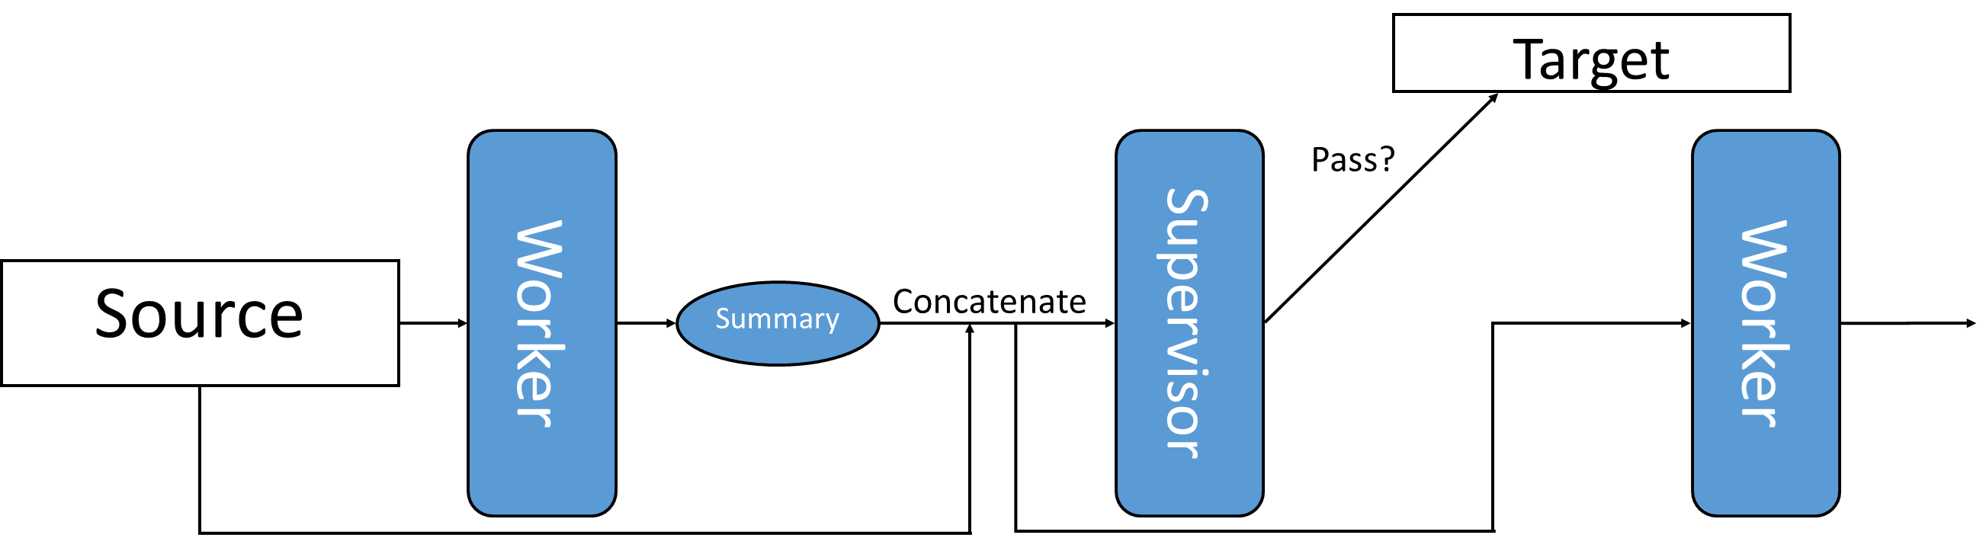
\includegraphics[scale=0.25]{architecture}
	\centering
	\caption{The worker-supervisor architecture}
\end{figure}

\subsection{Training the Model}
We train the model with the following procedure:
\begin{itemize}
	\item The worker is trained with a batch of sentence pairs from the training set.
	\item The supervisor is trained with a batch consisting of concatenated input and output sentence and a score of 0.99. Here we apply the label smoothing technique proposed by \cite{salimans2016improved} and avoid using the extreme values like 0 and 1.
	\item The worker is run to get a batch of inferred sentences.
	\item These sentences are concatenated with their source sentences, then sent to the supervisor with a score of 0.01. Similarly, 0 is an extreme value, so we use a less-extreme value of 0.01.
	\item These sentences are paired up with the actual target sentences, and then sent to the worker to train it.
\end{itemize}

For instance, if one sentence pair in the dataset is the following:

\begin{center}
	\begin{tabular}{p{57pt} p{170pt}}
		Source & a yale school of medicine study is expanding upon what scientists know about the link between schizophrenia and nicotine addiction .\\
		Truth Target & researchers examining evidence of link between schizophrenia and nicotine addiction
	\end{tabular}
\end{center}

We first train the worker on this sentence pair. Then we run the worker to generate a summary of the source sentence:
\begin{center}
	\begin{tabular}{p{57pt} p{170pt}}
		Model Output & yale study links schizophrenia
	\end{tabular}
\end{center}

We then concatenate this sentence with the source sentence, with a start of sentence token in-between to mark the start of the summary. Then we have created this training sentence pair ($<$sos$>$ denotes the start of sentence token):
\begin{center}
	\begin{tabular}{p{57pt} p{170pt}}
		New Source & a yale school of medicine study is expanding upon what scientists know about the link between schizophrenia and nicotine addiction . $<$sos$>$ yale study links schizophrenia\\
		Truth Target & researchers examining evidence of link between schizophrenia and nicotine addiction
	\end{tabular}
\end{center}

Then we train the worker again with this sentence pair. After both sentence pairs have been trained on the worker, we move on to the next sentence pair in the dataset.

\subsection{Running the Model}
The way to run the model is different than training because we allow the worker to retry the work multiple times, and a threshold score is used to determine whether the summarization needs to be redone.
\begin{itemize}
	\item The worker runs on the input sentence to generate an initial summary.
	\item The summary and the input sentence are concatenated and sent to the supervisor to obtain a score.
	\item If a score is greater than a specified threshold, then output the summary.
	\item Otherwise, the concatenated sentence is sent back to worker and repeat the steps above. These steps will only execute for at most a specified number of times.
\end{itemize}

\section{Environment Setup}
We used the Annotated English Gigaword corpus \cite{napoles2012annotated} as the training dataset, and DUC-2003 and DUC-2004 summarization tasks \cite{over2007duc} as the evaluation set. We followed the same preprocessing step as in the published NAMAS project \cite{rush2015neural}. We selected this preprocessing method because it has built-in tokenization and filters out bad sentence pairs that do not constitute a summary of the first sentence of that article.

We selected the GNMT system as the worker, and a multi-layer RNN with a fully-connected layer at the end as the supervisor. GNMT was originally built for the machine learning task, and its architecture is shown in Figure~\ref{fig:gnmt}. It features "residual connections" between LSTM layers. Residual connections are the summation of two consecutive layers' outputs, so that among every three consecutive layers, the input to the third layer is the sum of the output from the first two layers. It also uses three fully connected layers for the attention mechanism. This model has achieved great results with the translation task and is the underlying architecture of the Google Translate service inproduction. In our experiment, the worker was with TensorFlow and the supervisor is built using Keras with a TensorFlow backend. The encoder and decoder of GNMT and the supervisor have 8 layers of LSTM cells. We selected the batch size as 8 and spread the model across 8 GPUs. When concatenating sentences, we chose to retain the start-of-sentence token and the end-of-sentence token, because we thought these were clues for the encoder to realize this is a rework of a summarized sentence.

\begin{figure}[h]
	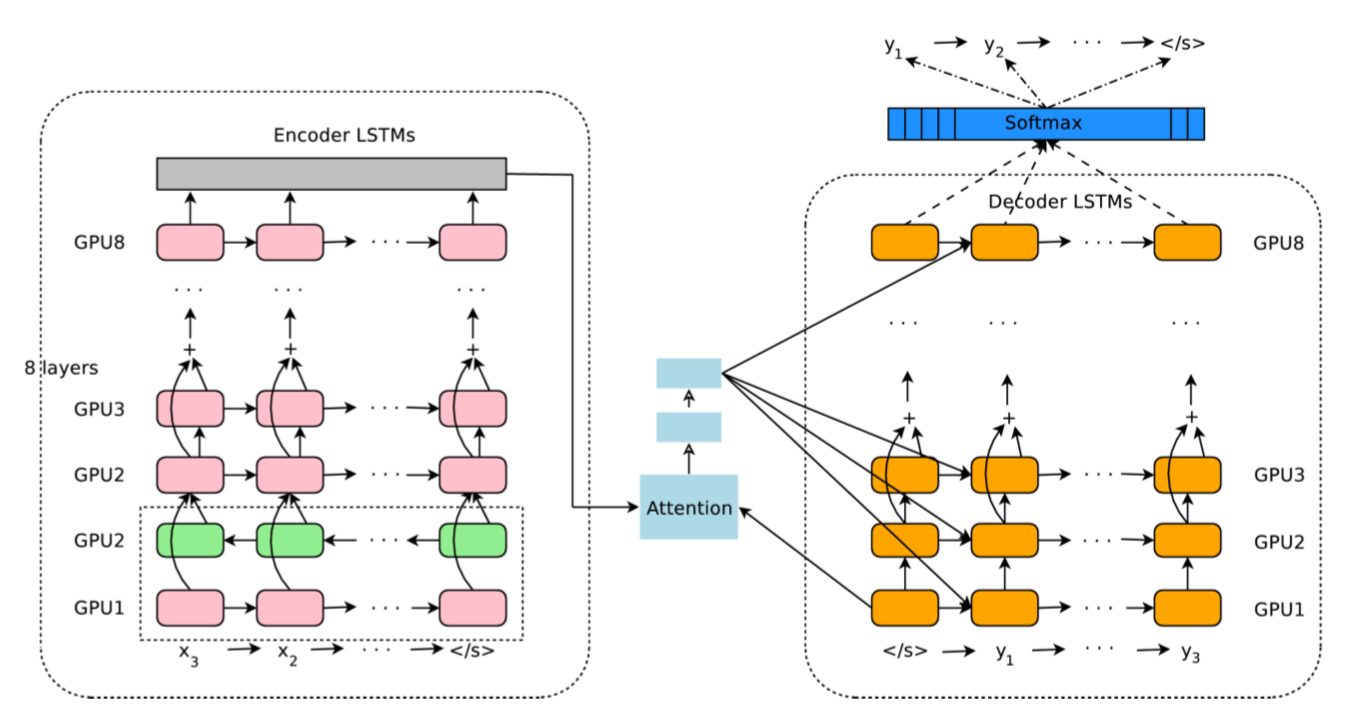
\includegraphics[scale=0.355]{GNMT}
	\centering
	\caption{GNMT architecture overview \cite{johnson2016google}}
	\label{fig:gnmt}
\end{figure}

We also tailored the system to the summarization task. We configured the model to use a shared vocabulary for both its encoder and decoder in order to reflect the idea that text summarization is comparable to a translation task from the source language to itself. Nonetheless, we decided to keep the embedding for the encoder and decoder to be separate, because a word should be able to convert into different vectors during encoding time and decoding time, because the nature of encoding and decoding are different.

During the initial training, we noticed that the training loss on concatenated source sentence decreased more rapidly than the loss on original source sentences. This is not beneficial because without a reasonable summary of the original source, the concatenation of source and summary does not provide more information than just the source itself. Therefore, we introduced a delay for the start of training with concatenated sentences. To address the rapid decrease of training loss with concatenated sentences more directly, we implemented a training guard which, when enabled, only trains the model with concatenated sentences when its last training loss is at least 2/3 of the training loss on original source sentences. Lastly, in order to compare the effect of delaying the training of the supervisor on the supervisor performance, we implemented a configurable delay of starting the training of the supervisor as well.

We prepared 5 systems for later evaluation. We use the NAMAS system as the baseline created by \cite{rush2015neural}, whose architecture is shown in Figure~\ref{fig:namas}. NAMAS is specially constructed for the DUC text summarization task, which we also used as the evaluation task. It features a smaller architecture than that of GNMT. It only uses one fully-connected layer for the attention mechanism, and does not use residual connections. However, it uses a beam search decoder rather than a greedy one. A greedy decoder picks the word with highest probability at each decoding step, but the beam search algorithm keeps k candidates with top probabilities, and keep finishing decoding using each of the candidates, so it produces the highest combined probability of the entire sentence. Moreover, the researchers at Facebook used Z-Mert tuning to further tune the model after it is trained, so its performance is probably higher than reported in this paper.

In our setup, NAMAS is trained with batch size of 64, embedding dimension of 64, Bag-of-Words dimension of 64, 64 LSTM cells per layer, initial learning rate of 0.1, and 20 epochs to reflect the reported setup in the original report. The modified GNMT system has 8 layers, each with 1024 LSTM cells, and a batch size of 64. We tested 3 sets of hyper-parameters using the Worker-Supervisor architecture, which are: 1. with the training guard enabled, start training with concatenated sentences at step 500, and start training the supervisor at step 200; 2. with the training guard enabled, start training with concatenated sentences at step 100, and start training the supervisor from the beginning; 3. with the training guard enabled, start training with concatenated sentences at step 10,000, and start training the supervisor at step 10,200. These will be referred to as WS-1, WS-2, and WS-3. During inference, we selected the rework threshold to be 0.5 and the maximum retries to be 10. Retry will be attempted when the discriminator score is lower than that threshold, but we cap the number of reattempts at 10.

\begin{figure}[h]
	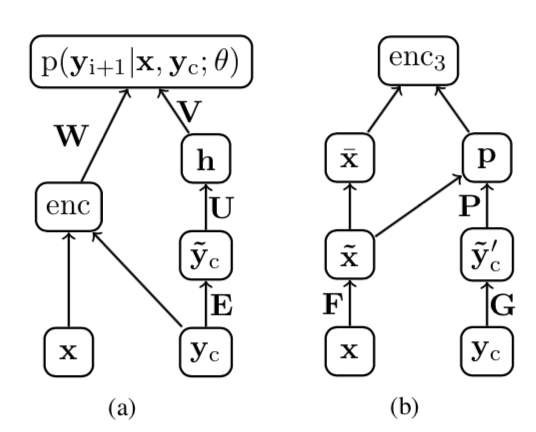
\includegraphics[scale=0.6]{NAMAS}
	\centering
	\caption{NAMAS architecture overview \cite{rush2015neural}}
	\label{fig:namas}
\end{figure}

\section{Results}
We used the ROUGE 2.0 system \cite{ganesan2015rouge} to evaluate our outputs with summaries produced by human summarizers. By default, this system evaluates with ROUGE-N (N-gram based) and ROUGE-L (summary level LCS). More specifically, ROUGE-N includes unigram (ROUGE-1) and bigram (ROUGE-2) . We will report the results for all the above metrics on the DUC-2003 and DUC-2004 summarization tasks separately.

Overall, due to time and resource constraint, the 5 systems are trained with different number of steps. NAMAS finished training 15 epochs. GNMT finished training 6,900 steps. WS-1 finished training 21,3500 steps. WS-2 finished training 20,9300 steps. Lastly, WS-3 finished training 11,0600 steps.

\subsection{DUC-2003}
The ROUGE 2.0 evaluation of DUC-2003 yields the results in Table~\ref{table:rougeduc2003}. The name "WS-N Source" refers to the n-th setup of the Worker-Supervisor model decoding with only the source sentence, which is also the initial summary. Likewise, "WS-N Concat" refers to n-th setup of the Worker-Supervisor model decoding with concatenated source sentence and initial summary. Furthermore, "RA" refers to the Read-Again baseline, and "RS" refers to the Reversed-Source setup. The baseline NAMAS model performs better than all other systems, followed by WS-1 with source only.

\begin{table}[h]
	\begin{tabular}{c c c c}
		Model & ROUGE-1 & ROUGE-2 & ROUGE-L \\
		\hline
		WS-1 Source & 28.650 & 4.158 & 27.94 \\
		WS-1 Concat & 22.411 & 3.012 & 23.557 \\
		WS-2 Source & 26.257 & 3.986 & 24.742 \\
		WS-2 Concat & 21.435 & 2.851 & 20.224 \\
		WS-3 Source & 20.273 & 2.215 & 18.112 \\
		WS-3 Concat & 1.882 & 0.151 & 2.541 \\
		\hline
		NAMAS & 39.228 & 9.183 & 39.903 \\
		GNMT & 32.789 & 5.909 & 33.580 \\
		RA Source & 34.143 & 6.611 & 34.931 \\
		RA Concat & 37.208 & 7.667 & 37.233 \\
		RS Source & 37.207 & 7.474 & 36.924 \\
		RS Concat & 37.856 & 7.544 & 37.467 \\
	\end{tabular}
	\caption{ROUGE 2.0 evaluation results on DUC-2003 summarization task}
	\label{table:rougeduc2003}
\end{table}

There are some sample summaries from this task:

\begin{table}[h]
	\begin{tabular}{p{40pt} p{170pt}}
		Source & fbi director louis freeh , believing his agency 's credibility is in question , wants someone from outside the bureau to examine whether his agents helped set the deadly blaze at the branch davidian compound near waco in 1993 , an agency spokesman said tuesday .\\
		\hline
		WS-1 Source & fbi chief says he is out of deadly oil \\
		WS-1 Concat & bp says it is out of oil spill \\
		WS-2 Source & after \#\# years of $<$unk$>$ $<$unk$>$ \\
		WS-2 Concat & fbi chief says he is not a $<$unk$>$ \\
		WS-3 Source & man 's death of the death of the death \\
		WS-3 Concat & $<$unk$>$  $<$unk$>$  $<$unk$>$  to death $<$unk$>$  \\
		NAMAS & fbi director says waco questioned \\
		GNMT & fbi director says fbi 's role in cia probe \\
		RA Source & fbi chief says fbi has n't been a $<$unk$>$ \\
		RA Concat & fbi director wants fbi to investigate fbi \\
		RS Source & fbi director wants fbi to investigate fbi \\
		RS Concat & fbi director wants fbi to investigate fbi \\
		\hline
		Ref 1 & FBI Director wants independent investigation of deadly Waco blaze.\\
		Ref 2 & Director wants outside investigation of FBI's role in Waco fire.\\
		Ref 3 & FBI director calls for independent investigation of Waco incident.\\
		Ref 4 & FBI director asks for independent probe of Waco; congress seeking evidence
	\end{tabular}
	\caption{Sample summaries on DUC-2003 summarization task}
	\label{table:sampleduc2003}
\end{table}

\subsection{DUC-2004}
The ROUGE 2.0 evaluation of DUC-2004 yields the results in Table~\ref{table:rougeduc2004}. Like the result for DUC-2003, the baseline NAMAS model performs better than all other systems, followed by WS-1 with source only.

\begin{table}[h]
	\begin{tabular}{c c c c}
		Model & ROUGE-1 & ROUGE-2 & ROUGE-L \\
		\hline
		WS-1 Source & 34.613 & 6.061 & 30.515 \\
		WS-1 Concat & 27.431 & 4.225 & 25.742 \\
		WS-2 Source & 30.969 & 4.656 & 27.895 \\
		WS-2 Concat & 25.516 & 3.618 & 22.618 \\
		WS-3 Source & 23.369 & 3.410 & 19.324 \\
		WS-3 Concat & 2.985 & 0.063 & 2.648 \\
		\hline
		NAMAS & 40.190 & 9.730& 39.074 \\
		GNMT & 40.19 & 8.021 & 37.443 \\
		RA Source & 42.928 & 10.089 & 40.25 \\
		RA Concat & 40.236 & 9.266 & 37.578 \\
		RS Source & 44.007 & 9.931 & 40.579 \\
		RS Concat & 41.67 & 9.425 & 37.131 \\
	\end{tabular}
	\caption{ROUGE 2.0 evaluation results on DUC-2004 summarization task}
	\label{table:rougeduc2004}
\end{table}

There are some sample summaries from this task:

\begin{table}[h]
	\begin{tabular}{p{40pt} p{170pt}}
		Source & king norodom sihanouk has declined requests to chair a summit of cambodia 's top political leaders , saying the meeting would not bring any progress in deadlocked negotiations to form a government . \\
		\hline
		WS-1 Source & indian pm says no change of political crisis \\
		WS-1 Concat & indian pm says no crisis talks to end crisis \\
		WS-2 Source & nepal 's top party holds to end political political \\
		WS-2 Concat & nepal 's party to hold political political parties \\
		WS-3 Source & malaysia 's party minister to hold talks with political \\
		WS-3 Concat & $<$unk$>$ $<$unk$>$ to $<$unk$>$ $<$unk$>$ to $<$unk$>$ $<$unk$>$ \\
		NAMAS & king sihanouk refuses to meet \\
		GNMT & king $<$unk$>$ cambodia 's top leaders \\
		RA Source & king sihanouk declines to chair of cambodia 's top political leaders \\
		RA Concat & king sihanouk <unk> cambodia 's king \\
		RS Source & king sihanouk denies cambodia 's top political leaders \\
		RS Concat & king <unk> cambodia 's top political leaders \\
		\hline
		Ref 1 & Sihanouk refuses to chair Cambodian political summit at home or abroad\\
		Ref 2 & Sihanouk refuses to host talks of Cambodian political leaders in Beijing.\\
		Ref 3 & Efforts to form a government deadlocked, Sihanouk will not chair summit\\
		Ref 4 & Norodom Sihanouk declines role to mediate in Cambodian governmental crisis
	\end{tabular}
	\caption{Sample summaries on DUC-2004 summarization task}
	\label{table:sampleduc2004}
\end{table}

\section{Discussions}
Overall, the evaluation results have shown that the GNMT system and the WS systems based on it failed to generate better summaries than the NAMAS system. NAMAS yield the top scores in all ROUGE metrics for both DUC-2003 and DUC-2004 summarization tasks. Furthermore, it was hard to determine whether the failure results from the weakness of the GNMT system with respect to the text summarization task. The pure GNMT model was significantly under-trained, so even though it did not generate better summaries than NAMAS, the reason can be considered mainly due to lack of training time, rather than the difference in the architectures.

Furthermore, reattempting the summary did not yield better results either. From the evaluation results, ROUGE scores dropped when the model was run on the concatenated sentence. In fact, this trend keeps going with more retries (TODO add figure). During the later retries, within a combined sentence, only the summary portion was replaced with the summary from the last attempt, so the total length did not necessarily grow with more attempts. Therefore, this ineffectiveness should probably be caused by the weakness of the architecture rather than a growing input sentence.

There are a few characteristics with the generated summaries that are worth noting too. In both examples above, the NAMAS system tends to focus on the wrong aspect of the source sentence, or just omit too much in formation. In the first example, all human summarizers focused on the independent investigation on FBI operation, but the NAMAS system focused on the "questioning" of the incident, which was more of a reason explaining the need of independent investigation. In the second example, the NAMAS system omitted entirely the objects of the meeting - top leaders in Cambodia, effectively resulting in a lack of important information.

Looking back at the summaries that GNMT and WS system produced, it is interesting that these models seems to not remember the "hard knowledge". In the second example, GNMT related King Sihanouk to Philippine, WS-1 related him to India, WS-2 related him to Nepal, and WS-3 related him to Malaysia, whereas his true nationality was Cambodia. On the contrary, NAMAS avoided summarizing this by just using the name "King Sihanouk". Although it was shown that the GNMT models understood that King Sihanouk was a leader of a country, they failed to associate him with the correct country.

Specifically with the concatenation technique, it seemed that the model output was more strongly affected by the later portion of the input, which may have led to worse reattempted summaries. This problem manifested itself with the WS-1 system in first example. After the initial summary made a mistake about "out of oil", the reattempt outputted "bp" as the subject of the sentence, completely ignoring the original subject, which was the FBI director. This could be indications that even though LSTM has shown higher performance when dealing with long sentences, it still weights later words more than earlier words. IAs a result, placing the source sentence in the beginning can lead to its information fading out from LSTM states This could be the reason that having "oil" has the last word of the sentence led to the mentioning of BP, a fuel company, and no information relating to FBI or director showed up in the reattempted summary, even though the source sentence is much longer than the first summary.

\section{Conclusion}
It has been seen that the proposed Worker-Supervisor architecture with concatenation is not more effective compared to the existing systems. However, based on the result obtained in the evaluations, we think there are ways to potentially improve the model.

In order to address the issue where the LSTM honors words that appear later in the sentence than those that appear earlier, it is possible that by reversing the order of the source and the summary.

Although neural machine translation models are similar to text summarization models, special designs can still bring improvements
Can try reversing the order of concatenation (i.e. Summary + Source instead of Source + Summary)
Have separate model handles Source and Source + Summary, then use the supervisor to select the better summary

\bibliography{References}
\bibliographystyle{aaai}
\end{document}
